




% サーバ側には独立したバックエンドシステムとの連携を容易でありWebアプリケーションがバックエンドシステムとの親和性が高く、
% より高い可用性とスケーラビリティを実現するができるREST APIを採用した.REST APIは、
% 複数のクライアントからアクセスができるため,様々なデバイスやプラットフォームからアクセスできる。これにより、より広いユーザー層からアクセスができる
% 既存の滞在ウォッチのサーバ側のシステムはpythonを用いて構築されており,動的型付け言語なため保守性が低いものであった.
% そこで静的型付けであり,高速な処理能力と小さなメモリフットプリントを持つため、Web APIの開発に適しているGolangを採用した.
% またGolangは並列処理を容易に実現できるため、高負荷な環境でのWeb APIの開発にも適している。さらに、標準パッケージによるHTTPサーバのサポートを持つため、
% Web APIの開発に必要な機能を簡単に実装できる。
% これらの特徴から、Golangを使用したWeb APIの開発は、高速でスケーラブルなAPIを提供することができ、開発効率も高い

\section{安定運用に向けた既存システムの再構築}\label{4.1}

既存の滞在ウォッチは長期に渡り継続的に保守・開発していくのが困難だったため安定運用を目指す上でシステムの再構築を行った.
4.1.1章では,サーバ側のシステムの再設計を行い,4.1.2章ではクライアント側のシステムの再設計を行った.





\subsection{サーバ側システムの再設計と再構築}\label{4.1.1}
サーバ側には独立したバックエンドシステムとの連携が容易かつWebアプリケーションのより高い可用性とスケーラビリティが実現できるREST APIを採用した.
REST APIは,多種多様なクライアントからアクセスができるため,様々なデバイスやプラットフォームからアクセスできる.
これにより,より広いユーザー層からアクセスが期待できる.


滞在ウォッチのサーバ側システムはPythonで構築されていたが,高負荷環境でパフォーマンスに影響を与える可能性があったのと動的型付け言語の開発,保守のしづらさを解消するため,Go言語を使用してシステムの再構築を行った.
Web APIは大量の処理をする必要があり,
Pythonの実行速度の遅さが,高負荷環境でパフォーマンスに影響を与える可能性がある.
また動的型付け言語なため,型の不明確さによってバグが見つけづらく保守性が低い.
そこで静的型付けであり,高速な処理能力と小さなメモリフットプリントを持つため,Web APIの開発に適しているGo言語を採用した.
Go言語は高いパフォーマンスを持つ.C言語のような低レベルな言語と
同等のパフォーマンスを持ちながら,高水準の言語のような簡単な構文を持っているのに加え,並列処理を容易に実現できるため,
高負荷な環境でのWeb APIの開発にも適している.
そのため,WebAPIの要求に適合する十分なパフォーマンスを提供できる.
また構造体とインターフェース型を備えており,WebAPIの開発に必要な柔軟性を持っている.これにより,開発者は,WebAPIを実装するために適した方法を選択できる.さらに,標準パッケージによるHTTPサーバのサポートを持つため,Web APIの開発に必要な機能を簡単に実装できる.

サーバで使用するデータベースは無料で利用でき,高いスケーラビリティを持つため,WebAPIの要求に対応可能なMySQLを採用した.MySQLは多くのプラットフォームでサポートされており,多くの言語に対応しており,開発者にとって選択肢が広がる.またMySQLは優れたセキュリティ機能を持つため,WebAPIのセキュリティの確保ができる.

Go言語でMySQLの操作を行う際Go言語のORMライブラリであるGormを採用した.
ORMはデータベースを操作を行うための手法の一つである.これによりデータベース操作を行う際に,SQL文を直接記述する必要がなくなりコードがすっきりし可読性が高くなる.
またSQL文を直接記述しないためSQLインジェクション対策にもなる.SQLインジェクションとは不正なSLQ文の挿入を行い,データベースに対して攻撃を行う手法である.ORMはプログラマが入力したデータを自動的にエスコープし,サイバー攻撃につながるような文字を無効化するためSQLインジェクション攻撃を防止できる.
GormはGo言語向けORMライブラリの一つである.Gormはデータベースの挿入,更新,削除,検索などの基本的な機能操作をサポートしている.また自動的なマイグレーション機能を持っている.これにより開発者はデータベーススキーマを手動で管理せずに,スキーマの変更を自動的に反映できる.
GoのORMライブラリとして他にXormなどの選択肢もあったが複雑なクエリを簡単に作成するための豊富なクエリビルダーAPIを提供しているためGormを選択した.

後述\ref{4.2}項で述べる利用者の管理とアクセス制御システムを実装するために,データベースにUserテーブルとRolesテーブルを新しく作成した.表\ref{table:users}と\ref{table:roles}にそれらのスキーマを示す.
既存のシステムでは存在していなかったemailプロパティとrole\_idプロパティを追加した.
emailプロパティは管理者が利用者のemailを登録すると保存される.\ref{4.3}で解説するがこのemail存在するかで利用者の認証を行う.role\_idはrolesテーブルの主キーである.rolesテーブルには管理者と一般利用者の2つのロールが存在する.役割の名前の変更や役割名が追加された場合にも対応できるようにrolesテーブルを作成している.



\begin{table}[]
  \caption{Usersテーブル}
  \centering
  \scalebox{1.4}{
    \begin{tabular}{|l|l|l|}
      \hline
      プロパティ & 型       & 説明                            \\ \hline
      id         & bigint   & 主キー                          \\ \hline
      name       & longtext & 名前                            \\ \hline
      uuid       & longtext & 使用者のビーコンのUUID          \\ \hline
      email      & longtext & email                           \\ \hline
      role\_id   & bigint   & 外部キー(rolesテーブルの主キー) \\ \hline
      create\_at & datetime & 作成日時                        \\ \hline
      update\_at & datetime & 更新日時                        \\ \hline
      delete\_at & datetime & 削除日時                        \\ \hline
    \end{tabular}}  \label{table:users}
\end{table}


\begin{table}[]
  \caption{Rolesテーブル}
  \centering
  \scalebox{1.4}{
    \begin{tabular}{|l|l|l|}
      \hline
      プロパティ & 型       & 説明                 \\ \hline
      id         & longtext & 主キー               \\ \hline
      name       & longtext & 役割の名前           \\ \hline
      create\_at & datetime & ユーザ情報の作成日時 \\ \hline
      update\_at & datetime & ユーザ情報の更新日時 \\ \hline
      delete\_at & datetime & ユーザ情報の削除日時 \\ \hline
    \end{tabular}
  }\label{table:roles}
\end{table}


サーバサイドプログラムの開発及びデプロイメントする際にはプログラムを実行するために必要な全ての環境をコンテナ内にパッケージ行い,
開発環境と本番環境での環境差を最小限に抑えられるDockerを採用した.
Dockerを使用すれば,アプリケーションを実行するために必要な全ての依存関係を内蔵したイメージを作成できる.これにより開発者はアプリケーションを実行するために必要な環境を1つのイメージにまとめられ,任意の環境に簡単に展開でき開発環境の構築が容易になる.
さらにDockerは他のアプリケーションの影響を受けずに実行可能である.
これによりアプリケーションが依存しているライブラリやフレームワークのバージョンなどの環境の違いによって,アプリケーションが動作しないといった問題を回避できる.
またコンテナを水平にスケールアウトできるため,アクセスが集中した場合にもスムーズな処理を行える.
デプロイ先は研究室内のサーバを利用した.研究室内のサーバの利用はクラウドサービスに比べて長期的にコストを削減できる.








\subsection{クライアントサイドの実装}\label{4.1.2}
クライアントサイドでは,WebAPIを利用して,Webアプリケーションを実装した.
Webアプリケーションのフレームワークとして,Next.jsを採用した.
Next.jsはReact.jsをベースにしており,React.jsの開発を効率化に加え,サーバーサイドによるレンダリングをサポートによるSEO対策やパフォーマンスの向上を実現できる.
React.jsはJavaScriptのライブラリであり,コンポーネントベースのアーキテクチャを採用している.
コンポーネントを独立した単位として開発すると,開発者はそれぞれのコンポーネントに集中できるため開発効率が向上する.
コンポーネントは再利用可能な単位であり複数のページで同じコンポーネントを利用することができ,これにより開発コストを削減し保守性を向上させる.
またReactは仮想DOMを採用しており実際のDOM(Document Object Model)を操作する代わりに、JavaScriptのオブジェクトとして扱う仕組みである.
仮想DOMは実際のDOMと比較して,更新が必要な部分だけを計算を行うためパフォーマンスの向上が図れる.



基本的に既存の滞在ウォッチで同じように滞在者,滞在画面,利用者情報のページが存在する.
変更点として在室者情報をガントチャートで滞在時間を可視化している画面が挙げられる.
部屋情報ごとのガントチャートが表できるようになっている.

\begin{figure}[tbh]
  \centering
  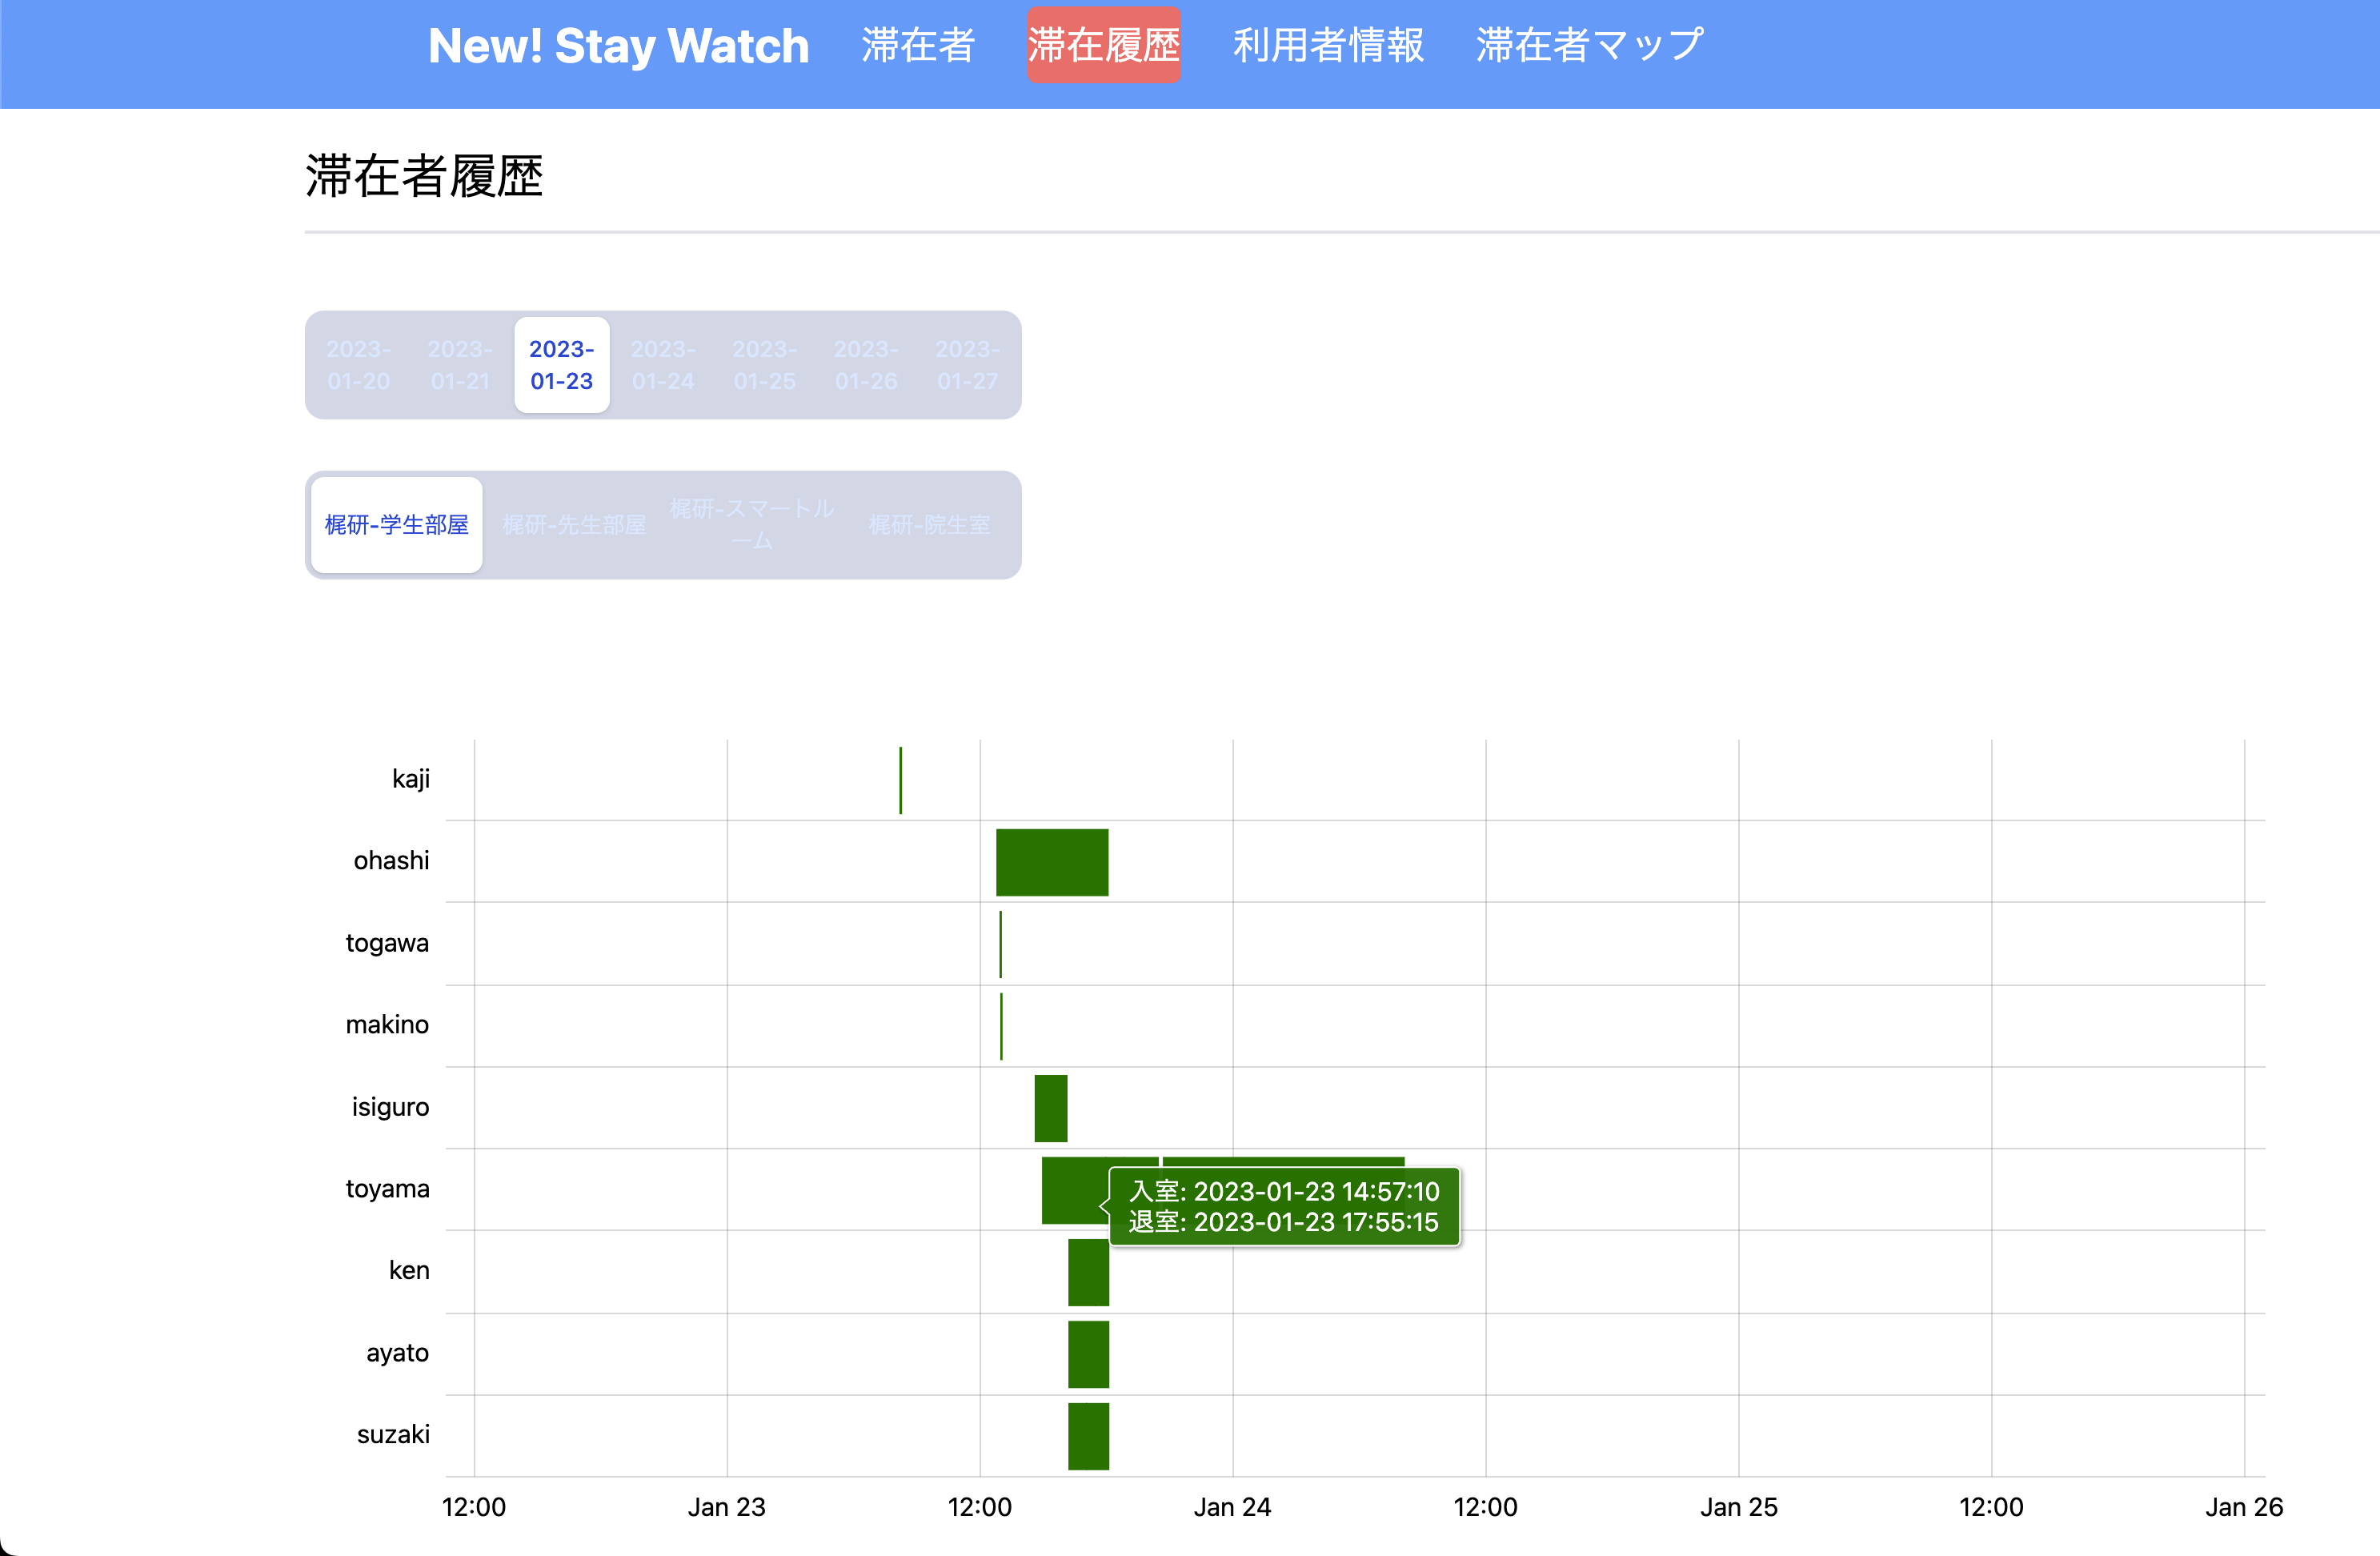
\includegraphics[width=16cm]{image/gantt.jpg}
  \caption{BLEビーコン登録済みの登録画面} \label{fig:gantt}
\end{figure}

























